
\documentclass[a4paper,11pt]{article}
\usepackage[a4paper, margin=8em]{geometry}

% usa i pacchetti per la scrittura in italiano
\usepackage[french,italian]{babel}
\usepackage[T1]{fontenc}
\usepackage[utf8]{inputenc}
\frenchspacing 

% usa i pacchetti per la formattazione matematica
\usepackage{amsmath, amssymb, amsthm, amsfonts}

% usa altri pacchetti
\usepackage{gensymb}
\usepackage{hyperref}
\usepackage{standalone}

% imposta il titolo
\title{Appunti Calcolo Numerico}
\author{Luca Seggiani}
\date{2025}

% disegni
\usepackage{pgfplots}
\pgfplotsset{width=10cm,compat=1.9}

% imposta lo stile
% usa helvetica
\usepackage[scaled]{helvet}
% usa palatino
\usepackage{palatino}
% usa un font monospazio guardabile
\usepackage{lmodern}

% tikz in sans
\tikzset{every picture/.style={/utils/exec={\sffamily}}}

\renewcommand{\rmdefault}{ppl}
\renewcommand{\sfdefault}{phv}
\renewcommand{\ttdefault}{lmtt}

% circuiti
\usepackage{circuitikz}
\usetikzlibrary{babel}

% disponi il titolo
\makeatletter
\renewcommand{\maketitle} {
	\begin{center} 
		\begin{minipage}[t]{.8\textwidth}
			\textsf{\huge\bfseries \@title} 
		\end{minipage}%
		\begin{minipage}[t]{.2\textwidth}
			\raggedleft \vspace{-1.65em}
			\textsf{\small \@author} \vfill
			\textsf{\small \@date}
		\end{minipage}
		\par
	\end{center}

	\thispagestyle{empty}
	\pagestyle{fancy}
}
\makeatother

% disponi teoremi
\usepackage{tcolorbox}
\newtcolorbox[auto counter, number within=section]{theorem}[2][]{%
	colback=blue!10, 
	colframe=blue!40!black, 
	sharp corners=northwest,
	fonttitle=\sffamily\bfseries, 
	title=Teorema~\thetcbcounter: #2, 
	#1
}

% disponi definizioni
\newtcolorbox[auto counter, number within=section]{definition}[2][]{%
	colback=red!10,
	colframe=red!40!black,
	sharp corners=northwest,
	fonttitle=\sffamily\bfseries,
	title=Definizione~\thetcbcounter: #2,
	#1
}

% disponi problemi
\newtcolorbox[auto counter, number within=section]{problem}[2][]{%
	colback=green!10,
	colframe=green!40!black,
	sharp corners=northwest,
	fonttitle=\sffamily\bfseries,
	title=Problema~\thetcbcounter: #2,
	#1
}

% disponi codice
\usepackage{listings}
\usepackage[table]{xcolor}

\definecolor{codegreen}{rgb}{0,0.6,0}
\definecolor{codegray}{rgb}{0.5,0.5,0.5}
\definecolor{codepurple}{rgb}{0.58,0,0.82}
\definecolor{backcolour}{rgb}{0.95,0.95,0.92}

\lstdefinestyle{codestyle}{
	backgroundcolor=\color{black!5}, 
	commentstyle=\color{codegreen},
	keywordstyle=\bfseries\color{magenta},
	numberstyle=\sffamily\tiny\color{black!60},
	stringstyle=\color{green!50!black},
	basicstyle=\ttfamily\footnotesize,
	breakatwhitespace=false,         
	breaklines=true,                 
	captionpos=b,                    
	keepspaces=true,                 
	numbers=left,                    
	numbersep=5pt,                  
	showspaces=false,                
	showstringspaces=false,
	showtabs=false,                  
	tabsize=2
}

\lstdefinestyle{shellstyle}{
	backgroundcolor=\color{black!5}, 
	basicstyle=\ttfamily\footnotesize\color{black}, 
	commentstyle=\color{black}, 
	keywordstyle=\color{black},
	numberstyle=\color{black!5},
	stringstyle=\color{black}, 
	showspaces=false,
	showstringspaces=false, 
	showtabs=false, 
	tabsize=2, 
	numbers=none, 
	breaklines=true
}

\lstdefinelanguage{javascript}{
	keywords={typeof, new, true, false, catch, function, return, null, catch, switch, var, if, in, while, do, else, case, break},
	keywordstyle=\color{blue}\bfseries,
	ndkeywords={class, export, boolean, throw, implements, import, this},
	ndkeywordstyle=\color{darkgray}\bfseries,
	identifierstyle=\color{black},
	sensitive=false,
	comment=[l]{//},
	morecomment=[s]{/*}{*/},
	commentstyle=\color{purple}\ttfamily,
	stringstyle=\color{red}\ttfamily,
	morestring=[b]',
	morestring=[b]"
}

% disponi sezioni
\usepackage{titlesec}

\titleformat{\section}
{\sffamily\Large\bfseries} 
{\thesection}{1em}{} 
\titleformat{\subsection}
{\sffamily\large\bfseries}   
{\thesubsection}{1em}{} 
\titleformat{\subsubsection}
{\sffamily\normalsize\bfseries} 
{\thesubsubsection}{1em}{}

% disponi alberi
\usepackage{forest}

\forestset{
	rectstyle/.style={
		for tree={rectangle,draw,font=\large\sffamily}
	},
	roundstyle/.style={
		for tree={circle,draw,font=\large}
	}
}

% disponi algoritmi
\usepackage{algorithm}
\usepackage{algorithmic}
\makeatletter
\renewcommand{\ALG@name}{Algoritmo}
\makeatother

% disponi numeri di pagina
\usepackage{fancyhdr}
\fancyhf{} 
\fancyfoot[L]{\sffamily{\thepage}}

\makeatletter
\fancyhead[L]{\raisebox{1ex}[0pt][0pt]{\sffamily{\@title \ \@date}}} 
\fancyhead[R]{\raisebox{1ex}[0pt][0pt]{\sffamily{\@author}}}
\makeatother

\begin{document}

% sezione (data)
\section{Lezione del 16-05-25}

% stili pagina
\thispagestyle{empty}
\pagestyle{fancy}

% testo

\subsection{Intervallo di convergenza}
Vorremo estendere la definizione di convergenza data in 19.2 in un certo intervello $[a, b]$.

Iniziamo con un esempio:
\subsubsection{Esempio: convergenza del metodo di Newton}
Prendiamo la funzione:
$$
f(x) = 3 x^2 e^{-x} - 1
$$
e poniamo:
$$
f(x) = 0
$$
cioè equivalentemente uguagliamo le due funzioni:
$$
3x^2 = e^x
$$
che sono rispettivamente una parabola simmetrica rispetto all'asse $y$ e un esponenziale.

Queste intersezioni saranno 3, che chiamiamo $\alpha_{1, 2, 3}$.
Avremo che, scelti i punti $x_{0, 1, 2}$:
$$
x_0 = -\frac{1}{2}, \quad x_1 = 1, \quad x_2 = 5
$$
si avrà la convergenza nei rispettivi punti $\alpha_{1, 2, 3}$.

\subsubsection{Convergenza in un intervallo}
Una domanda che potremo farci, in relazione all'ultimo esempio, è quando possiamo assicurare che un metodo converge $\forall x_0 \in [a, b]$.

Esiste il seguente teorema:
\begin{theorem}{Teorema di convergenza in un intervallo}
	Se $\phi(x) \in C^1 ([a, b])$ e:
	\begin{enumerate}
		\item $|\phi'(x)| < 1, \quad \forall x \in [a, b]$;
		\item $\phi(x) \in [a, b], \quad \forall x \in [a, b]$;
	\end{enumerate}
	allora $\phi(x)$ converge su $[a, b]$.
\end{theorem}
Dove l'ipotesi in più rispetto al teorema di convergenza locale (teorema 19.2) è la 2.

\subsubsection{Condizioni di convergenza globale per Newton}
Nello specifico per Newton, la convergenza in un intervallo si assicura attraverso condizioni su concavità e convessità.

Esiste infatti il seguente teorema:
\begin{theorem}{Convergenza globale per Newton}
	Se $\alpha \in [a, b]$ è radice semplice di $f \in C^2([a, b])$, e $f, f''$ sono di segno costante su $[a, b]$, il metodo di Newton converge globalmente in maniera superlineare ($\geq 2$) $\forall x_0$ che verifica:
	$$
	f(x_0) \cdot f''(x_0) > 0
	$$
\end{theorem}
Dove si mette enfasi su \textit{globalmente}, in quanto il teorema 20.1 ha valenza solo locale.
Sostanzialmente, questo teorema ci è utile per fare stime iniziali, probabilmente arbitrariamente distanti dall'origine, che convergano con velocità superlinare.

Osserviamo che:
\begin{itemize}
	\item Se la funzione è \textbf{concava}, chiediamo $f(x_0) < 0$;
	\item Se la funzione è \textbf{convessa}, chiediamo $f(x_0) > 0$.
\end{itemize}

In particolare distinguiamo quindi i 4 casi:
\begin{enumerate}
	\item $f' > 0$, $f'' > 0$ convessa crescente, vorremo partire a \textit{destra} di $\alpha$;
	\item $f' < 0$, $f'' > 0$ convessa decrescente, vorremo partire a \textit{sinistra} di $\alpha$;
	\item $f' > 0$, $f'' < 0$ concava crescente, vorremo partire a \textit{sinistra} di $\alpha$;
	\item $f' < 0$, $f'' < 0$ concava decrescente, vorremo partire a \textit{destra} di $\alpha$;
\end{enumerate}

\newpage

Cioè riassumendo:
\begin{table}[h!]
	\center 
	\begin{tabular} { c | c c }
		& $f'(x) > 0$ & $f'(x) < 0$ \\
		\hline
		$f''(x) > 0$      
		&
		\raisebox{-\totalheight}{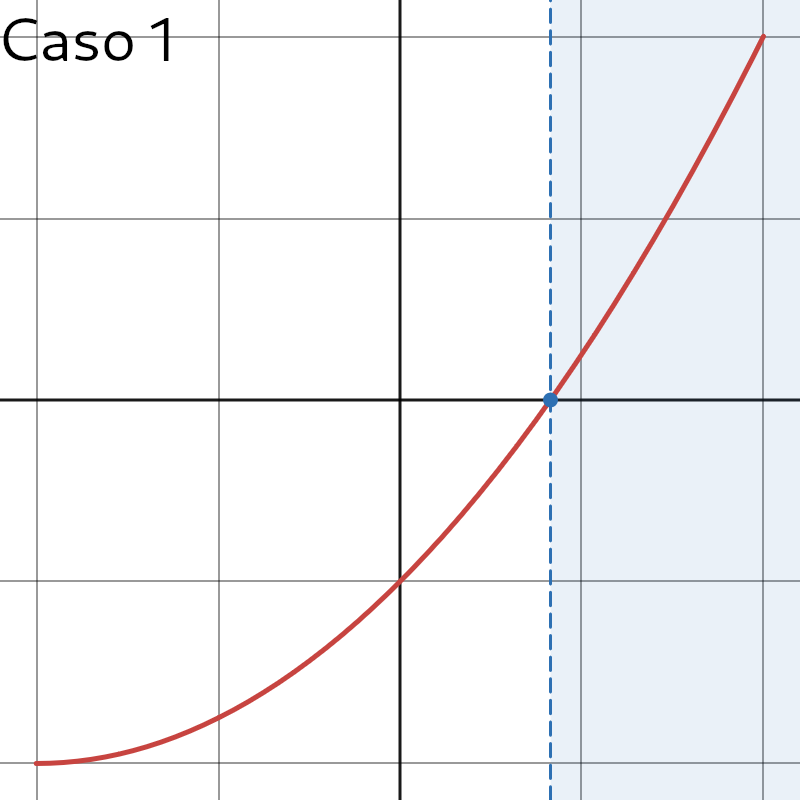
\includegraphics[scale=0.2]{../figures/newton_conv/case_1.png}} 
		& 
		\raisebox{-\totalheight}{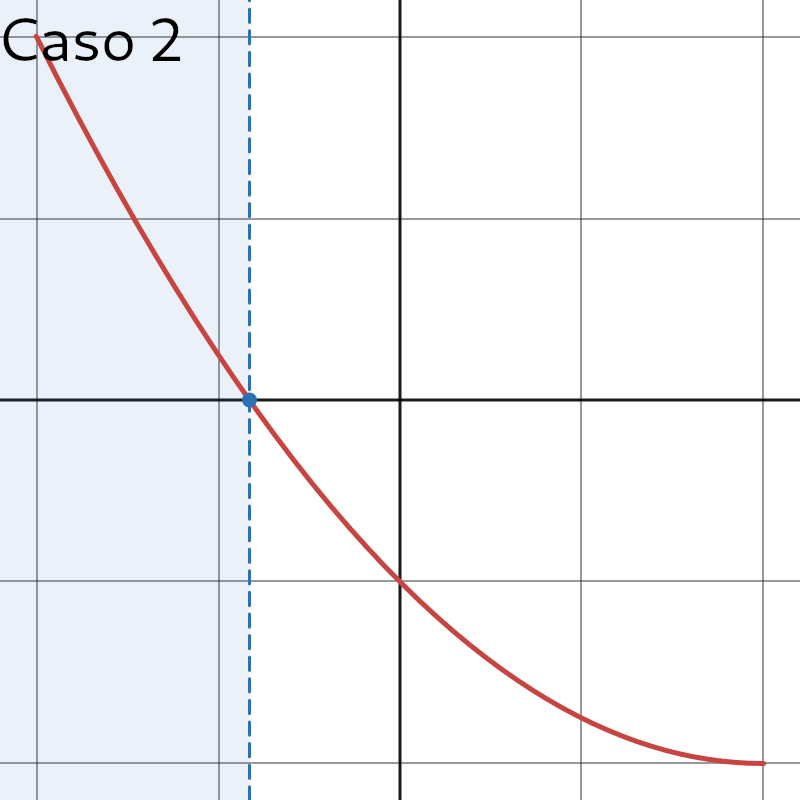
\includegraphics[scale=0.2]{../figures/newton_conv/case_2.png}} 
		\\
		$f''(x) < 0$
		&
		\raisebox{-\totalheight}{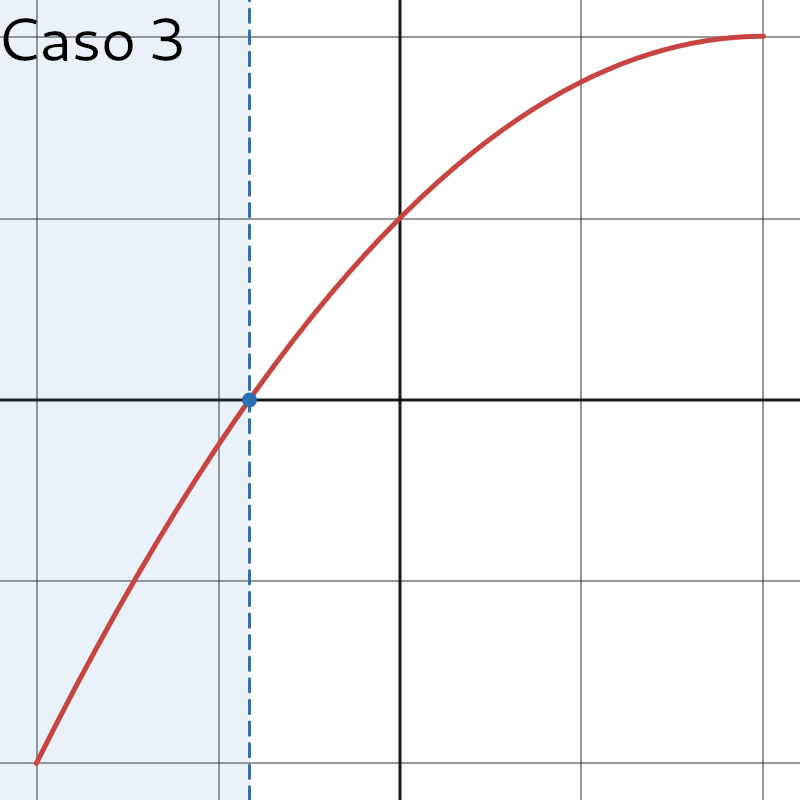
\includegraphics[scale=0.2]{../figures/newton_conv/case_3.png}} 
		& 
		\raisebox{-\totalheight}{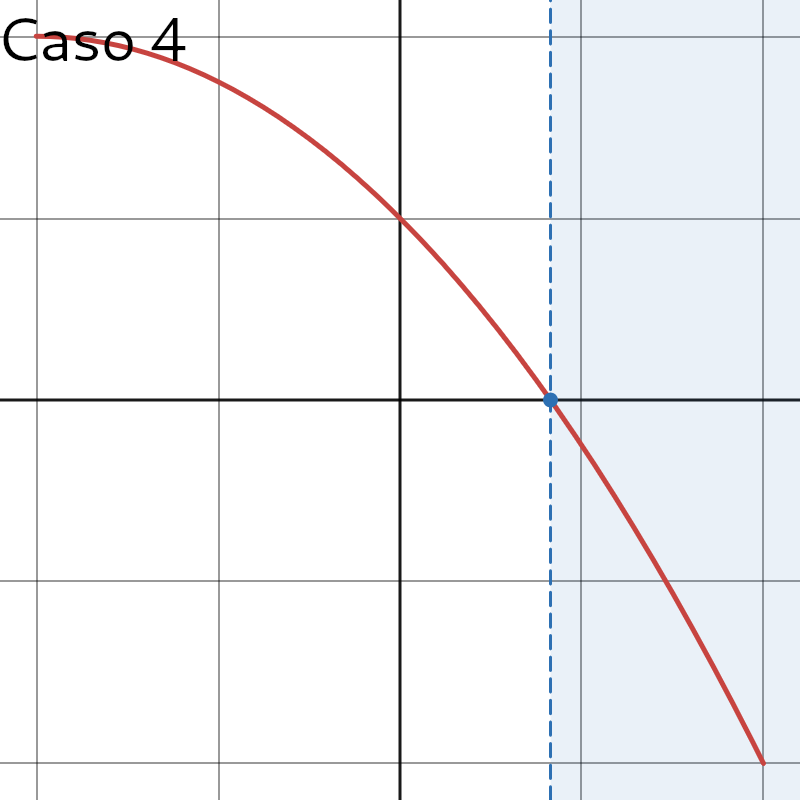
\includegraphics[scale=0.2]{../figures/newton_conv/case_4.png}} 
		\\
	\end{tabular}
\end{table}

\subsubsection{Esempio: ricerca di un intervallo di convergenza}
Prendiamo la funzione:
$$
f(x) = x + \log(x)
$$
e cerchiamo un intervallo dove questa ha una radice, in particolare fornendo un punto di partenza $x_0$ per cui Newton risulta convergente.

Chiaramente quello che cerchiamo sono le intersezioni dei grafici:
$$
\log(x) = -x
$$
che saranno una sola, compresa fra 0 e 1, perciò:
$$
\alpha \in (0, 1)
$$

Vediamo quindi se si applicano le condizioni di convergenza per Newton.
Calcoliamo innanzitutto le derivate:
$$
f'(x) = 1 + \frac{1}{x}, \quad > 0 \text{ su } (0, 1)
$$
$$
f''(x) = -\frac{1}{x^2}, \quad < 0 \text{ su } (0, 1)
$$

Per $1$ la condizione non è soddisfatta, in quanto si troverà a \textit{destra} di $\alpha$ (e trovandoci nel caso 3, vorremo prendere punti a \textit{sinistra}).

Dovremo quindi cercare un $x_0 \in (0, \alpha)$, ovvero $x_0 : f(x_0) < 0$.
Proviamo $\frac{1}{e}$:
$$
f\left(\frac{1}{e}\right) = \frac{1}{e} - 1 < 0
$$
per cui possiamo scegliere $x_0 = \frac{1}{e}$ ed essere sicuri, per il teorema 21.2, di convergere ad $\alpha$.

\subsection{Equazioni non lineari in $\mathbb{R}^m$}
Vediamo quindi di considerare sempre equazioni non lineari, ma in più variabili (in particolare $m$).

Cercheremo quindi $f(x) = 0$ per $f: \mathbb{R}^m \rightarrow \mathbb{R}^m$, cioè:
$$
f =
\begin{pmatrix}
	f_1 (x_1, ..., x_m) \\
	\vdots \\
	f_m (x_1, ..., x_m) \\
\end{pmatrix}
$$
e vorremo trovare $\alpha \in \mathbb{R}^m$, cioè:
$$
\alpha = 
\begin{pmatrix}
	\alpha_1 \\
	\vdots \\
	\alpha_m
\end{pmatrix}
$$
tale che:
$$
f(\alpha) = 
\begin{pmatrix}
	f_1 (\alpha_1, ..., \alpha_m) \\
	\vdots \\
	f_m (\alpha_1, ..., \alpha_m) \\
\end{pmatrix}
= 0
$$

Questo problema corrisponde effettivamente a cercare soluzioni a sistemi di $m$ equazioni in $m$ incognite, non lineari.

\par\smallskip

In particolare, ci può essere utile per trovare i punti stazionari di funzioni in più variabili, ovvero le soluzioni di $\nabla F(x) = 0$, con $F(x) : \mathbb{R}^m \rightarrow \mathbb{R}$ cioè:
$$
\nabla F(x) = 
\begin{pmatrix}
	\frac{\partial }{\partial x_1} F(x_1, ..., x_m) \\
	\vdots \\ 
	\frac{\partial }{\partial x_m} F(x_1, ..., x_m) \\
\end{pmatrix}
$$

\par\smallskip

Nel caso dei sistemi lineari, avevamo la condizione semplice:
$$
f(x) = b - Ax, \quad x = A^{-1} b
$$
mentre in questo caso non avremo a disposizione tali semplificazioni.

Ci potremo quindi chiedere come risolvere $f(x)$ nel caso non lineare.
La soluzione sarà quella di generalizzare i metodi di punto fisso a $\mathbb{R}^m$, definendoli come:
$$
x = \phi(x), \quad \phi : \mathbb{R}^m \rightarrow \mathbb{R}^m
$$
e quindi usare la solita formula di aggiornamento:
$$
x^{(n + 1)} = \phi(x^{(n)})
$$

Una possibile formula di aggiornamento può essere:
$$
\phi(x) = x - G(x) \cdot f(x)
$$
dove $G(x)$ è:
$$
G(x) : \mathbb{R}^m \rightarrow \mathbb{R}^{m \times m}
$$
cioè:
$$
G(x) =
\begin{pmatrix}
	G_{11}(x) & ... & G(1m)(x) \\
	\vdots & \vdots & \vdots \\
	G_{m1}(x) & ... & G(mm)(x) \\
\end{pmatrix}
$$
e si cerca $G(x)$ tale che $G(\alpha)$ è non singolare, ovvero 
$$
\det(G(\alpha)) \neq 0
$$
Quindi si considera l'iterazione:
\[
	\begin{cases}
		x^{(0)} \in \mathbb{R}^m, \quad \text{dato} \\
		x^{(n + 1)} = x^{(n)} - G(x^{(n)}) f(x^{(n)}) = \phi (x^{(n)})
	\end{cases}
\]

Ridiamo la definizione di convergenza in $\mathbb{R}^n$:
\begin{definition}{Convergenza multivariabile}
	La successione $\{x^{(n)}\}_{n \in \mathbb{N}}$ converge ad $\alpha \in \mathbb{R}^m$ se:
	$$
	\lim_{n \rightarrow + \infty} | x^{(n)} - \alpha|_2 = 0
	$$
\end{definition}

In particolare, la convergenza ha \textbf{ordine} $p > 0$ se vale:
$$
\lim_{n \rightarrow +\infty} \frac{|x^{(n + 1)} - \alpha|_2}{|x^{(n)} - \alpha|_2^p} = c 
$$
con $c \neq 0$, $c < +\infty$, e in particolare nel caso $p = 1$ è $C \in (0, 1)$, cioè si ha la stessa situazione della definizione 19.3.

\par\smallskip

Nel caso esistano e siano continue le derivate delle componenti di $\phi(x)$ si introduce il \textbf{Jacobiano} di $\phi$, come la funzione $J_\phi : \mathbb{R}^m \rightarrow \mathbb{R}^{m \times m}$ definita da:
$$
J_\phi(x) = 
\begin{pmatrix}
	\frac{\partial \phi_1}{\partial x_1}(x) & ... & \frac{\partial \phi_1}{\partial x_m}(x) \\
	\vdots & \vdots & \vdots \\
	\frac{\partial \phi_m}{\partial x_1}(x) & ... & \frac{\partial \phi_m}{\partial x_m}(x) \\
\end{pmatrix}
$$
oppure per componenti:
$$
[J_\phi(x)]_{ij} = \frac{\partial \phi_i}{\partial x_j} (x), \quad i, j = 1, ..., m
$$

Potremo quindi enunciare il seguente teorema:
\begin{theorem}{Convergenza locale multivariabile}
	Sia $\phi(x) \in C^1(\Omega)$, $\Omega \subseteq \mathbb{R}^m$ con $\alpha \in \Omega$ tale che $\phi(\alpha) = \alpha$.
	Se:
	$$
	\rho\left(J_\phi (\alpha) \right) < 1
	$$
	cioè il raggio spettrale del Jacobiano di $\phi$ in $\alpha$ è $< 1$, allora $\exists \delta > 0$ tale che:
	$$
	\forall x^{(0)} : |x^{(0)} - \alpha|_2 < \delta
	$$
	in cui la successione:
	$$
	x^{(n + 1)} = \phi(x^{(n)})
	$$
	converge ad $\alpha$, ed $\alpha$ è l'unico punto fisso di $\phi$ in:
	$$
	\{ z \in \mathbb{R}^m : |z - \alpha|_2 < \delta \}
	$$
\end{theorem}

Osserviamo quindi che se per una qualsiasi norma si trova che:
$$
| J_\phi(\alpha) | < 1
$$
allora vale la tesi del teorema, ovvero la convergenza locale.
Viceversa, se si trova che:
$$
| J_\phi(\alpha) | \geq 1
$$
non si può concludere nulla.

\subsubsection{Esempio: convergenza multivariabile}
Prendiamo la funzione, con $m = 2$:
$$
f(x_1, x_2) = 
\begin{pmatrix}
	x_1 - \frac{1}{4} (x_1^2 + x_2^2) \\
	x_2 + x_1 - 2
\end{pmatrix}
$$
e cerchiamone i punti $f(\alpha) = 0$, cioè che soddisfano:
\[
	\begin{cases}
		x_1 - \frac{1}{4} (x_1^2 + x_2^2) = 0 \\
		x_2 + x_1 - 2 = 0
	\end{cases}
\]

Dalla $f$, posto $f(x) = 0$ si derivano le identità:
\[
	\begin{cases}
		x_1 = \frac{1}{4} (x_1^2 + x_2^2)	\\
		x_2 = 2 - x_1
	\end{cases}
\]
per cui si può considerare $\phi(x)$:
$$
\phi(x) =
\begin{pmatrix}
	\frac{1}{4} (x_1^2 + x_2^2) \\
	2 - x_1
\end{pmatrix}
$$
e 
prendere l'aggiornamento dal metodo stazionario ad un punto:
$$
x^{(n + 1)} = \phi(x^{(n)})
$$

\par\smallskip

Prima di valutare la convergenza, cerchiamo di trovare i punti $\alpha$ in maniera analitica.

Per la prima equazione, avremo che:
$$
x - \frac{1}{4} (x^2 + y^2) = 0 \, \Rightarrow \, - \frac{(x - 2)^2}{4} - \frac{y^2}{4} + 1 = 0
$$
cioè si trova la circonferenza di centro $(2, 0)$ e raggio $2$.

Per la seconda, si ha invece semplicemente la retta:
$$
y = 2 - x
$$

Sul grafico, questo ha l'aspetto:
\begin{center}
	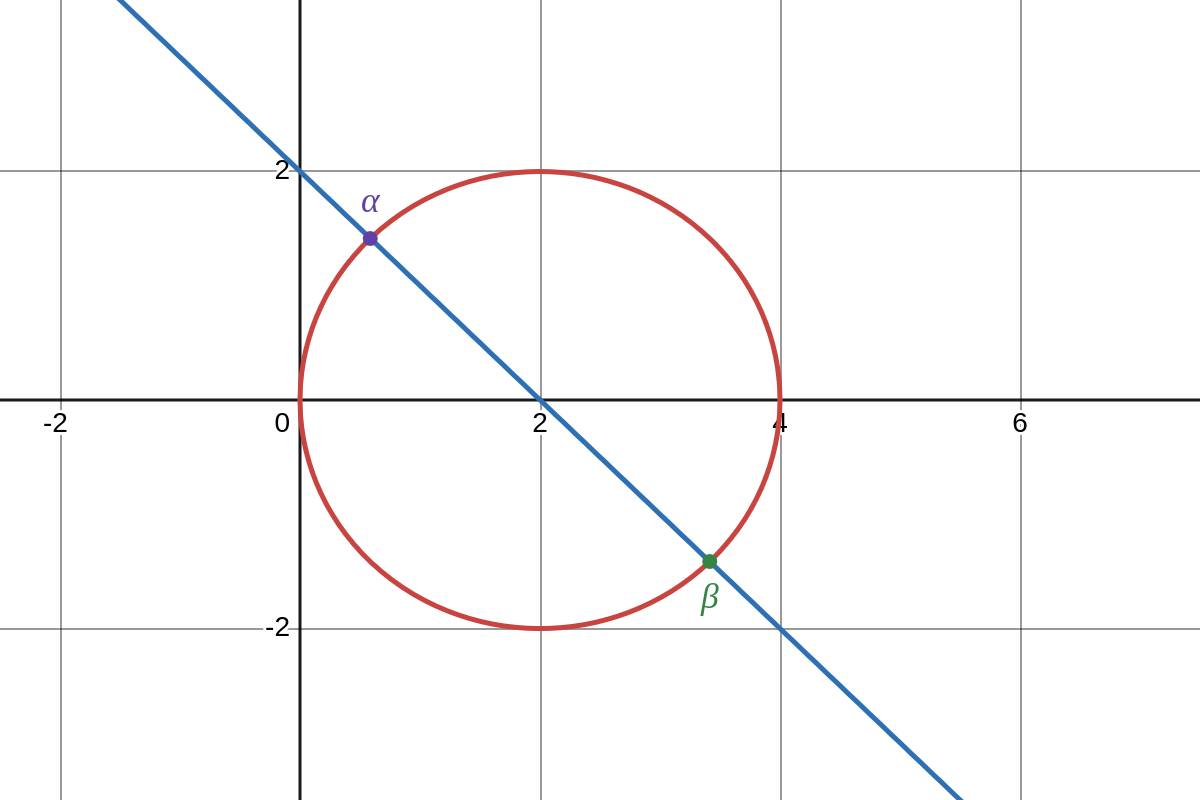
\includegraphics[scale=0.3]{../figures/nonlin.png}
\end{center}

Le soluzioni di $f(x) = 0$ saranno quindi i punti di intersezione fra la circonferenza e la retta, che vediamo essere 2, uno sopra l'asse $x$ e l'altro sotto.
Consideriamone solo il primo, che chiamiamo $(\alpha_1, \alpha_2)$.

\par\smallskip

Calcoliamo quindi il Jacobiano:
$$
J_\phi(x) =
\begin{pmatrix}
	\frac{x_1}{2} & \frac{x_2}{2} \\
	-1 & 0
\end{pmatrix}
$$

Vediamo che questa ha norma $\geq 1$, per cui bisogna calcolare gli autovalori.

Guardiamo quindi al polinomio caratteristico:
$$
\left(\frac{x_1}{2} - \lambda\right) \left(-\lambda\right) + \frac{x_2}{2} = \lambda^2 - \frac{x_1}{2} \lambda + \frac{x_2}{2} \rightarrow \lambda_{1, 2} = \frac{\frac{x_1}{2} \pm \sqrt{\frac{x_1^2}{4} - 2 x_2}}{2}
$$
cioè:
$$
\lambda_{1, 2} = \frac{\frac{\alpha_1}{2} \pm \sqrt{\frac{\alpha_1^2}{4} - 2 \alpha_2}}{2}
$$

Valutando la posizione generica di $\alpha$, si ha che:
$$
\alpha_1 < 1, \quad \alpha_2 \in (1, 2)
$$
che formalmente si ottiene notando che $\alpha_1 \geq 1$ porta ad un assurdo, e $\alpha_2 = 2 - \alpha_1$.

Da questo deriverà che il discriminante:
$$
\Delta = \frac{\alpha_1^2}{4} - 2 \alpha_2 < 0
$$
e cioè $\lambda_{1, 2}^\alpha$ sono necessariamente numeri complessi in forma:
$$
\lambda_{1, 2}^\alpha = \frac{\alpha_1}{4} \pm i \sqrt{ \frac{\alpha_2}{2} - \frac{\alpha_1^2}{16} }
$$

Il modulo di uno di questi (prendiamo il primo) sarà:
$$
|\lambda_1^\alpha|^2 = \frac{\alpha_1^2}{16} + \frac{\alpha_1}{2} - \frac{\alpha_1^2}{16} = \frac{\alpha_1}{2}
$$
per cui il raggio spettrale sarà $\frac{\alpha_1}{2} < 1$ (dal fatto che $\alpha_1 < 1$), e quindi il metodo convergente.

\subsubsection{Esempio: convergenza multivariabile con MATLAB}
Facciamo una trattazione meno analitica e più numerica della convergenza nello scorso esempio.

Avevamo individuato due radici, chiamiamole $\alpha$ (già ampiamente discussa) e $\beta$.
Queste si calcono esplicitamente prendendo dalla seconda equazione:
$$
x_2 + x_1 - 2 = 0 \implies x_2 = 2 - x_1
$$
e sostituendo nella prima:
$$
x_1 - \frac{1}{4} (x_1^2 + (2 - x_1)^2) = -\frac{x_1^2}{2} + 2 x_1 - 1
$$
da cui:
$$
\alpha = (2 - \sqrt{2}, \sqrt{2}), \quad \beta = (2 + \sqrt{2}, - \sqrt{2})
$$

Potremo chiaramente rifare le stesse considerazioni di prima con i valori effettivi di $\alpha$, trovando gli stessi risultati.
Ci basti sapere che il punto $\alpha$ fa (come avevamo visto) da attrattore, mentre il metodo non converge in $\beta$, scelto l'aggiornamento:
$$
\phi(x) =
\begin{pmatrix}
	\frac{1}{4} (x_1^2 + x_2^2) \\
	2 - x_1
\end{pmatrix}
$$

Vediamo di implementare in MATLAB un risolutore che applichi nella pratica tale funzione.
Questo si tradurrà nel dire:
\lstset{style=codestyle, language=MATLAB}
\lstinputlisting{../code/matlab/nonlin_r2_ex.m}

Dove notiamo che si stampano alcune informazioni intermedie sui punti attraversati, e si traccia il percorso seguito su un grafico.

\begin{itemize}
	\item Se si sceglie come punto di inizio $(1, 1)$, con l'intenzione di convergere ad $\alpha$, si ha il seguente andamento:
		\begin{center}
			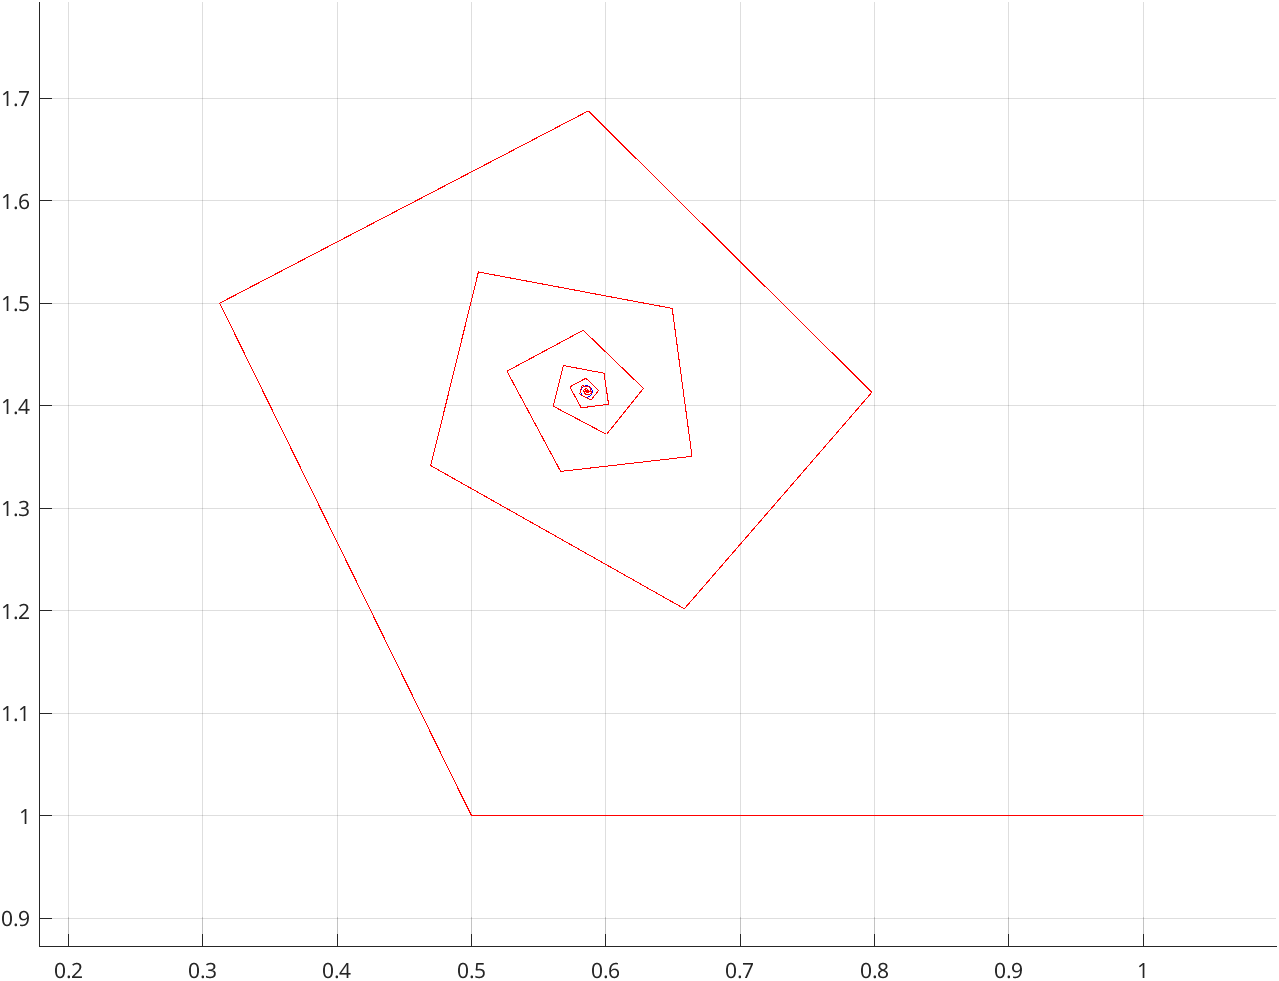
\includegraphics[scale=1]{../figures/nonlin_ex.png}
		\end{center}
		da dove si nota chiaramente che in un numero limitato di passaggi ci si avvicina abbastanza ad $\alpha$;
		\newpage
	\item Cercare di fare la stessa cosa ad esempio dal punto $(4, -1)$ non dà risultati simili, in quanto notiamo dal grafico:
		\begin{center}
			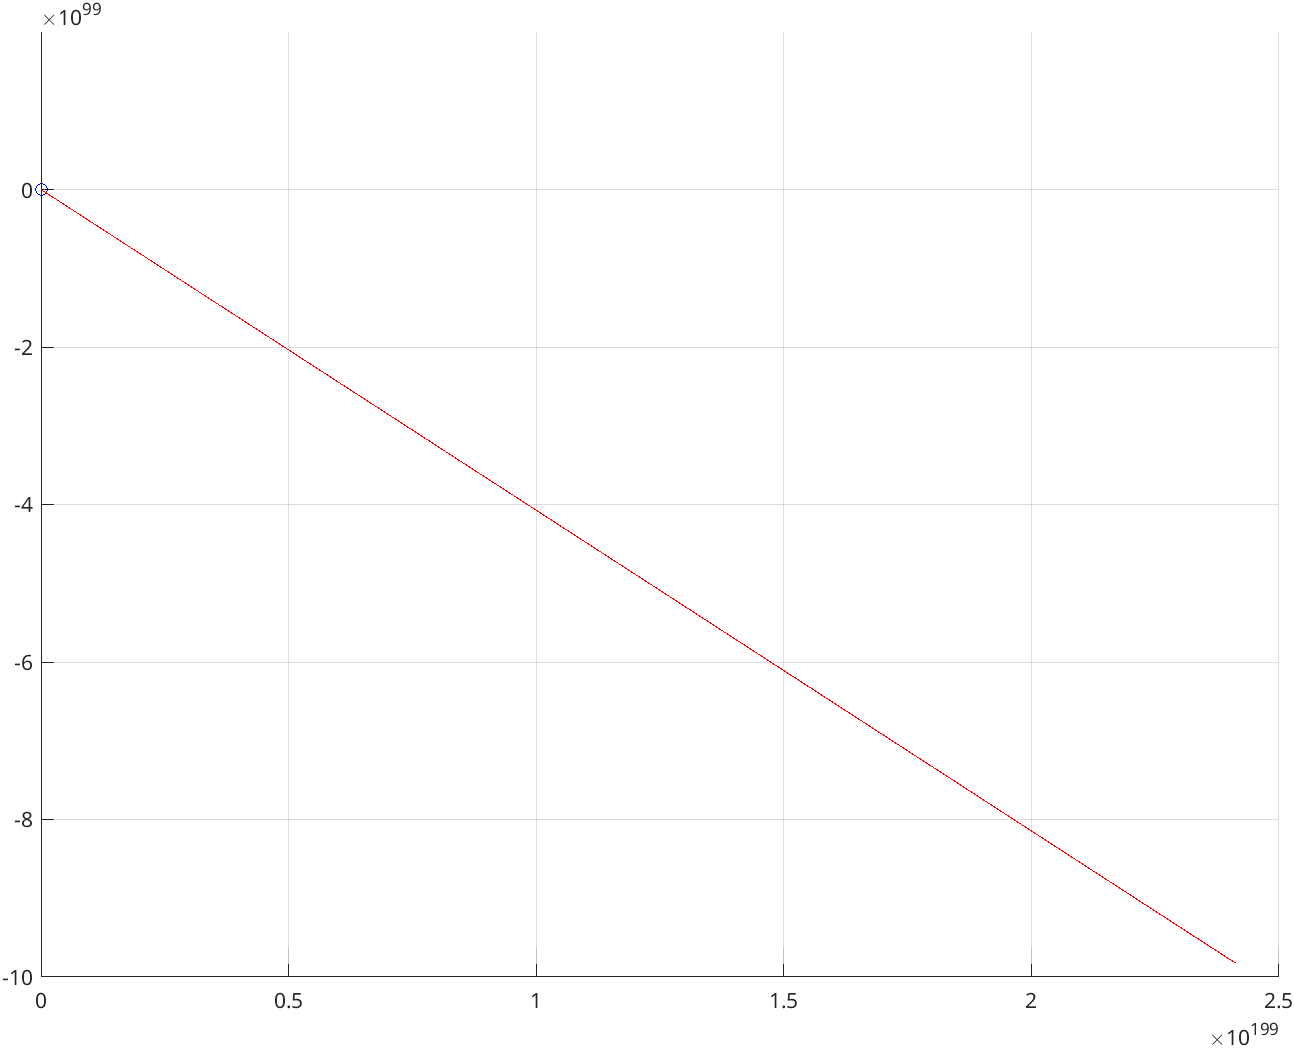
\includegraphics[scale=1]{../figures/nonlin_ex2.png}
		\end{center}
		che il risultato esplode velocemente all'infinito, e quindi chiaramente il metodo non converge.
\end{itemize}

\subsection{Metodo di Newton-Raphson}
Vediamo quindi la versione multivariabile del metodo di Newton-Raphson.

Quindi, se abbiamo $f : \mathbb{R}^m \rightarrow \mathbb{R}^m$ il metodo di Newton si generalizza nel seguente modo:
$$
x^{(n + 1)} = x^{(n)} - J_f (x^{(n)})^{-1} f(x^{(n)})
$$

Osserviamo che ad ogni passo si valuta $J_f(x^{(n)})$ e $f(x^{(n)})$, si risolve il sistema lineare:
$$
J_f(x^{(n)}) y = f(x^{(n)})
$$
ed infine si chiama $x^{(n + 1)} = x^{(n)} - y$.

L'aggiornamento complessivo sarà quindi:
\[
	\begin{cases}
		x^{(0)}, \quad \text{dato} \\
		x^{(n + 1)} = x^{(n)} - J_f(x^{(n)})^{-1} f(x^{(n)})
	\end{cases}
\]

Per quanto riguarda la convergenza si ha il seguente risultato:
\begin{theorem}{Convergenza del metodo di Newton-Rapson}
	Sia $f \in C^2(\Omega)$, $\Omega \subseteq \mathbb{R}^m$, $\alpha \in \Omega$ tale che $f(\alpha) = 0$.
	Se $J_f(\alpha)$ è non singolare, allora $\exists s \subseteq \Omega$ intorno di $\alpha$ tale che $\forall x^{(0)} \in S$ la successione generata dal metodo di Newton-Raphson a partire da $x^{(0)}$ converge e vale:
	$$
	|x^{(n + 1)} - \alpha|_2 \leq \beta |x^{(n)} - \alpha |_2^2
	$$
	ovvero la convergenza è almeno quadratica (quindi superlineare).
\end{theorem}

\subsubsection{Esempio: metodo di Newton-Raphson}
Vediamo quindi come valutare la convergenza del metodo di Newton-Raphson per il sistema:
$$
f(x_1, x_2) =
\begin{pmatrix}
	\frac{1}{3} (x_1 - x_2) + x_1^2 \\
	\frac{1}{3} (-x_1 + x_2) + x_1 x_2
\end{pmatrix}
$$

\par\smallskip

Vogliamo quindi determinare le radici di $f$, che si otterrano come:
\[
	\begin{cases}
		\frac{x_1 - x_2}{3} + x_1^2 = 0 \\
		\frac{x_2 - x_1}{3} + x_1 x_2 = 0
	\end{cases}
	\, \Rightarrow \,
	\begin{cases}
		x_2 = 3 x_1^2 + x_1 \\
		\left( \frac{- x_1 + x_1 + 3 x_1^2}{3} \right) + x_1 (3 x_1^2 + x_1) = 0
	\end{cases}
	\, \Rightarrow \,
	\begin{cases}
		x_2 = 3 x_1^2 + x_1 \\
		2x_1^2 + 3x_1^3 = 0
	\end{cases}
\]
da cui si ottengono i due punti:
$$
\alpha = \begin{pmatrix}
0 \\ 0
\end{pmatrix}, \quad
\beta = \begin{pmatrix}
	-\frac{2}{3} \\ \frac{2}{3}
\end{pmatrix}
$$

\par\smallskip

Vorremo quindi valutare il Jacobiano:
$$
J_f(x_1, x_2) =
\begin{pmatrix}
	\frac{1}{3} + 2 x_1 & -\frac{1}{3} \\
	-\frac{1}{3} + x_2 & \frac{1}{3} + x_1
\end{pmatrix}
$$

Che nei due punti $\alpha$ e $\beta$ risulta:
\begin{itemize}
	\item[$\alpha$]:
		$$
		J_f(\alpha) =
		\begin{pmatrix}
			\frac{1}{3} & -\frac{1}{3} \\ 
			-\frac{1}{3} & \frac{1}{3}
		\end{pmatrix}
		$$
		da cui $\det = 0$, e la convergenza non è superlineare;
	\item[$\beta$]:
		$$
		J_f(\beta) =
		\begin{pmatrix}
			-1 & -\frac{1}{3} \\ 
			\frac{1}{3} & -\frac{1}{3}
		\end{pmatrix}
		$$
		da cui $\det \neq 0$, e la convergenza è superlineare;
\end{itemize}

\subsubsection{Varianti del metodo di Newton-Raphson}
Abbiamo che ad ogni passo del metodo di Newton-Raphson dobbiamo:
\begin{enumerate}
	\item Valutare $J_f(x^n)$; ovvero $m^2$ funzioni non lineari;
	\item Risolvere $J_f(x^n) y = f(x^n)$, sistema lineare $m \times m$ (complessità $O(m^3))$.
\end{enumerate}

Quando $m$ è particolarmente grande siamo disposti a fare qualcosa di più economico al prezzo di perdere l'ordine di convergenza molto favorevole di Newton-Rhapson.

\begin{enumerate}
	\item La prima strategia è quella di non aggiornare mai il Jacobiano (\textbf{Newton semplificato}).
		Il Jacobiano viene quindi calcolato solo in $x^0$ punto iniziale, e poi si usa sempre lo stesso nelle iterazioni successive, cioè l'aggiornamento diventa:
		$$
			x^{n + 1} = x^n - J_f(x^0)^{-1} f(x^n)
		$$
		
		Per la risoluzione del sistema, si può quindi sfruttare la fattorizzazione $LU$ del Jacobiano appena nominato, e quindi svolgere complessivamente due operazioni $O(m^2)$.

	\item La seconda strategia viene detta \textbf{metodo di Jacobi nonlineare}.
		Ad ogni passo si sostituisce $J_f(x^n)$ con la matrice diagonale:
		$$
		\mathrm{diag} \left( \frac{\partial f}{\partial x_1} (x^n), ..., \frac{\partial f}{\partial x_m} (x^n) \right)
		$$
		così che:
		\begin{enumerate}
			\item Bisogna fare $m$ valutazioni di funzioni non lineari;
			\item Risolvere il sistema lineare costa $O(m)$.
		\end{enumerate}

		L'aggiornamento diventa quindi qualcosa del tipo:
		$$
		x_i^{n + 1} = x_i^n - \frac{f_i(x^n)}{\frac{\partial f}{\partial x_i} (x_1^n, ..., x_m^n)}
		$$

	\item La terza strategia viene detta \textbf{metodo di Gauss-Seidel nonlineare}.

		In questo caso l'aggiornamento è sostanzialmente analogo al metodo di Jacobi, con la differenza:
		$$
		x_i^{n + 1} = x_i^n - \frac{f_i(x_1^{n + 1}, ..., x_i^{n}, ... x_m^n)}{\frac{\partial f}{\partial x_i} (x_1^n, ..., x_m^n)}
		$$
		dove le entrate $x^{n + 1}$ vengono calcolate una per volta attraverso le stesse considerazioni fatte per il metodo di Gauss-Seidel lineare.
\end{enumerate}

Altre varianti sono date dai metodi \textbf{quasi-Newton}, dove si sostituisce $J_f(x)$ con qualcosa con cui è più semplice (meno costoso) risolvere sistemi lineari e che richiedono meno valutazioni di funzioni non lineari.

\end{document}
